\section{Singleton}

O padrão \textit{Singleton} garante que um objeto possuirá apenas uma 
instância. Além disso, fornece um único ponto acessível 
globalmente a essa instância. Esse padrão é útil 
para implementar classes que fornecem serviços sem que seja 
necessário instanciar vários objetos idênticos em 
locais diferentes do código.\cite{gamma:1995}

A Figura \ref{singleton_struct} demonstra a implementação 
do padrão. A classe \texttt{Singleton} possui um método construtor 
privado e armazena no atributo estático \texttt{uniqueInstance} uma 
instância de \texttt{Singleton}. Através do método de classe 
\texttt{Instance}, é verificado se já existe uma instância 
armazenada no atributo \texttt{uniqueInstance}. Caso já exista, 
ela é retornada. Caso não, a instância única é criada 
para ser retornada nas chamadas posteriores de \texttt{Instance}.

\begin{figure}[htb]
	\caption{\label{singleton_struct}Estrutura do \textit{Singleton}.}
	\begin{center}
	    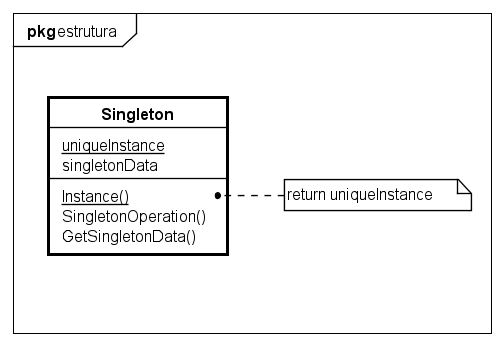
\includegraphics[scale=0.6]{5_padroes-contexto-funcional/5.1_criacionais/5.1.5_singleton/singleton_estrutura.png}
	\end{center}
  \caption*{Fonte: O Autor (2021)}
\end{figure}

\subsection*{Exemplo Orientado a Objetos}

Uma classe define as operações para realizar transações com 
uma base de dados. Como a instância dela é idêntica independente 
do cliente que a utiliza, não existe a necessidade de replicar 
essas instâncias pelo código. Ela pode ser transformada em 
um \textit{Singleton}, o que faz com que toda classe que deseja fazer 
uma transação na base de dados apenas solicite uma instância 
e realize as operações. A definição da classe do exemplo 
pode ser vista na Figura \ref{singleton_exemplo} e no 
Código \ref{oosingleton}.

\begin{figure}[htb]
	\caption{\label{singleton_exemplo}Exemplo de \textit{Singleton}.}
	\begin{center}
	    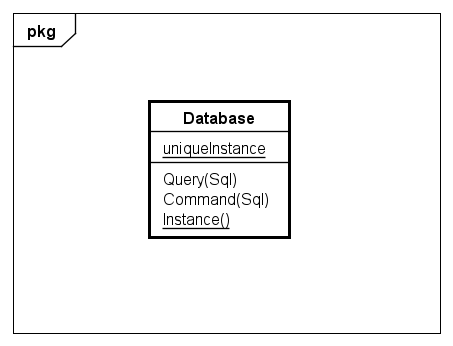
\includegraphics[scale=0.6]{5_padroes-contexto-funcional/5.1_criacionais/5.1.5_singleton/singleton_exemplo.png}
	\end{center}
  \caption*{Fonte: O Autor (2021)}
\end{figure}

\begin{lstlisting}[caption={\textit{Singleton} Orientação a Objetos.},label=oosingleton]

class Database private(){
  def Query(sql : String) : Object = {
    //Execute query
    null
  }
  def Command(sql : String) : Unit = {
    //Execute command
  }
}

object Database {
  private var instance : Database = null

  def Instance() : Database = {
    if(instance == null){
      instance = new Database()
    }
    instance
  }
}

\end{lstlisting}
\legend{Fonte: O Autor (2021)}

\subsection*{Contexto Funcional}

Em um contexto sem classes e objetos, 
um \textit{Singleton} poderia ser considerado como 
uma variável global, acessível por 
todo o programa. Essa ideia viola o conceito 
de função pura, já que uma função que acessa 
um \textit{Singleton} deixa de depender apenas de seus 
parâmetros. Para o caso em que o \textit{Singleton} 
armazene algum estado, o conceito de imutabilidade 
também precisaria ser violado, já que o 
valor que armazena o \textit{Singleton} precisaria ser 
mutável para ser alterado de dentro de uma 
função. Com isso, não existe uma implementação 
equivalente ao \textit{Singleton} no contexto funcional.